% Options for packages loaded elsewhere
\PassOptionsToPackage{unicode}{hyperref}
\PassOptionsToPackage{hyphens}{url}
\PassOptionsToPackage{dvipsnames,svgnames,x11names}{xcolor}
%
\documentclass[
  singlecolumn]{article}

\usepackage{amsmath,amssymb}
\usepackage{iftex}
\ifPDFTeX
  \usepackage[T1]{fontenc}
  \usepackage[utf8]{inputenc}
  \usepackage{textcomp} % provide euro and other symbols
\else % if luatex or xetex
  \usepackage{unicode-math}
  \defaultfontfeatures{Scale=MatchLowercase}
  \defaultfontfeatures[\rmfamily]{Ligatures=TeX,Scale=1}
\fi
\usepackage[]{libertinus}
\ifPDFTeX\else  
    % xetex/luatex font selection
\fi
% Use upquote if available, for straight quotes in verbatim environments
\IfFileExists{upquote.sty}{\usepackage{upquote}}{}
\IfFileExists{microtype.sty}{% use microtype if available
  \usepackage[]{microtype}
  \UseMicrotypeSet[protrusion]{basicmath} % disable protrusion for tt fonts
}{}
\makeatletter
\@ifundefined{KOMAClassName}{% if non-KOMA class
  \IfFileExists{parskip.sty}{%
    \usepackage{parskip}
  }{% else
    \setlength{\parindent}{0pt}
    \setlength{\parskip}{6pt plus 2pt minus 1pt}}
}{% if KOMA class
  \KOMAoptions{parskip=half}}
\makeatother
\usepackage{xcolor}
\usepackage[top=30mm,left=20mm,heightrounded]{geometry}
\setlength{\emergencystretch}{3em} % prevent overfull lines
\setcounter{secnumdepth}{-\maxdimen} % remove section numbering
% Make \paragraph and \subparagraph free-standing
\ifx\paragraph\undefined\else
  \let\oldparagraph\paragraph
  \renewcommand{\paragraph}[1]{\oldparagraph{#1}\mbox{}}
\fi
\ifx\subparagraph\undefined\else
  \let\oldsubparagraph\subparagraph
  \renewcommand{\subparagraph}[1]{\oldsubparagraph{#1}\mbox{}}
\fi


\providecommand{\tightlist}{%
  \setlength{\itemsep}{0pt}\setlength{\parskip}{0pt}}\usepackage{longtable,booktabs,array}
\usepackage{calc} % for calculating minipage widths
% Correct order of tables after \paragraph or \subparagraph
\usepackage{etoolbox}
\makeatletter
\patchcmd\longtable{\par}{\if@noskipsec\mbox{}\fi\par}{}{}
\makeatother
% Allow footnotes in longtable head/foot
\IfFileExists{footnotehyper.sty}{\usepackage{footnotehyper}}{\usepackage{footnote}}
\makesavenoteenv{longtable}
\usepackage{graphicx}
\makeatletter
\def\maxwidth{\ifdim\Gin@nat@width>\linewidth\linewidth\else\Gin@nat@width\fi}
\def\maxheight{\ifdim\Gin@nat@height>\textheight\textheight\else\Gin@nat@height\fi}
\makeatother
% Scale images if necessary, so that they will not overflow the page
% margins by default, and it is still possible to overwrite the defaults
% using explicit options in \includegraphics[width, height, ...]{}
\setkeys{Gin}{width=\maxwidth,height=\maxheight,keepaspectratio}
% Set default figure placement to htbp
\makeatletter
\def\fps@figure{htbp}
\makeatother
\newlength{\cslhangindent}
\setlength{\cslhangindent}{1.5em}
\newlength{\csllabelwidth}
\setlength{\csllabelwidth}{3em}
\newlength{\cslentryspacingunit} % times entry-spacing
\setlength{\cslentryspacingunit}{\parskip}
\newenvironment{CSLReferences}[2] % #1 hanging-ident, #2 entry spacing
 {% don't indent paragraphs
  \setlength{\parindent}{0pt}
  % turn on hanging indent if param 1 is 1
  \ifodd #1
  \let\oldpar\par
  \def\par{\hangindent=\cslhangindent\oldpar}
  \fi
  % set entry spacing
  \setlength{\parskip}{#2\cslentryspacingunit}
 }%
 {}
\usepackage{calc}
\newcommand{\CSLBlock}[1]{#1\hfill\break}
\newcommand{\CSLLeftMargin}[1]{\parbox[t]{\csllabelwidth}{#1}}
\newcommand{\CSLRightInline}[1]{\parbox[t]{\linewidth - \csllabelwidth}{#1}\break}
\newcommand{\CSLIndent}[1]{\hspace{\cslhangindent}#1}

\usepackage{cancel}
\usepackage[noblocks]{authblk}
\renewcommand*{\Authsep}{, }
\renewcommand*{\Authand}{, }
\renewcommand*{\Authands}{, }
\renewcommand\Affilfont{\small}
\usepackage{cancel}
\makeatletter
\makeatother
\makeatletter
\makeatother
\makeatletter
\@ifpackageloaded{caption}{}{\usepackage{caption}}
\AtBeginDocument{%
\ifdefined\contentsname
  \renewcommand*\contentsname{Table of contents}
\else
  \newcommand\contentsname{Table of contents}
\fi
\ifdefined\listfigurename
  \renewcommand*\listfigurename{List of Figures}
\else
  \newcommand\listfigurename{List of Figures}
\fi
\ifdefined\listtablename
  \renewcommand*\listtablename{List of Tables}
\else
  \newcommand\listtablename{List of Tables}
\fi
\ifdefined\figurename
  \renewcommand*\figurename{Figure}
\else
  \newcommand\figurename{Figure}
\fi
\ifdefined\tablename
  \renewcommand*\tablename{Table}
\else
  \newcommand\tablename{Table}
\fi
}
\@ifpackageloaded{float}{}{\usepackage{float}}
\floatstyle{ruled}
\@ifundefined{c@chapter}{\newfloat{codelisting}{h}{lop}}{\newfloat{codelisting}{h}{lop}[chapter]}
\floatname{codelisting}{Listing}
\newcommand*\listoflistings{\listof{codelisting}{List of Listings}}
\makeatother
\makeatletter
\@ifpackageloaded{caption}{}{\usepackage{caption}}
\@ifpackageloaded{subcaption}{}{\usepackage{subcaption}}
\makeatother
\makeatletter
\@ifpackageloaded{tcolorbox}{}{\usepackage[skins,breakable]{tcolorbox}}
\makeatother
\makeatletter
\@ifundefined{shadecolor}{\definecolor{shadecolor}{rgb}{.97, .97, .97}}
\makeatother
\makeatletter
\makeatother
\makeatletter
\makeatother
\ifLuaTeX
  \usepackage{selnolig}  % disable illegal ligatures
\fi
\IfFileExists{bookmark.sty}{\usepackage{bookmark}}{\usepackage{hyperref}}
\IfFileExists{xurl.sty}{\usepackage{xurl}}{} % add URL line breaks if available
\urlstyle{same} % disable monospaced font for URLs
\hypersetup{
  pdftitle={TESTS},
  pdfauthor={Joseph A. Bulbulia},
  pdfkeywords={DAGS, Causal
Inference, Confounding, History, Psychology, Panel},
  colorlinks=true,
  linkcolor={blue},
  filecolor={Maroon},
  citecolor={Blue},
  urlcolor={Blue},
  pdfcreator={LaTeX via pandoc}}

\title{TESTS}


  \author{Joseph A. Bulbulia}
            \affil{%
                  Victoria University of Wellington, New Zealand, School
                  of Psychology, Centre for Applied Cross-Cultural
                  Research
              }
      
\date{2023-07-30}
\begin{document}
\maketitle
\begin{abstract}
TEST
\end{abstract}
\ifdefined\Shaded\renewenvironment{Shaded}{\begin{tcolorbox}[interior hidden, enhanced, frame hidden, sharp corners, boxrule=0pt, borderline west={3pt}{0pt}{shadecolor}, breakable]}{\end{tcolorbox}}\fi

\hypertarget{measurement-error-in-the-confounder}{%
\subsubsection{Measurement Error in the
Confounder}\label{measurement-error-in-the-confounder}}

Measurement error pervades all research. Figure
Figure~\ref{fig-dag-measure-confounder} demonstrates that even
error-free measurements of the exposure and outcome cannot counteract
the bias in causal effect estimates introduced by measurement error in
the confounders. Accurate measurement of confounders mitigates threats
to confounding. Once more, conducting a sensitivity analysis is
essential to evaluate the potential impact of this threat.\footnote{A
  simple yet powerful form of sensitivity analysis involves the
  computation of E-Values. E-Values calculate the minimal strength of
  association that an unmeasured confounder would require with both the
  exposure and outcome, beyond the measured confounders, to negate the
  observed exposure-outcome association (refer to the R package
  \texttt{EValue}: (\protect\hyperlink{ref-mathur2018}{Mathur et al.
  2018})).}

\begin{figure}

{\centering \includegraphics[width=1\textwidth,height=\textheight]{test-again_files/figure-pdf/fig-dag-measure-confounder-1.pdf}

}

\caption{\label{fig-dag-measure-confounder}Causal diagram demonstrating
a confounder, L, measured with error, L'. Despite perfect measurements
of the exposure, A, and the outcome, Y, a bias-inducing (backdoor) path
opens between A - L - Y, highlighted in red. Given the ubiquity of
measurement error, it is imperative to minimise such errors and conduct
sensitivity analyses to assess the risk of unmeasured confounding.}

\end{figure}

\hypertarget{bias-reduction-by-conditioning-on-a-post-outcome-variable-to-diminish-directed-measurement-error-bias}{%
\subsubsection{Bias Reduction by Conditioning on a Post-outcome Variable
to Diminish Directed Measurement Error
Bias}\label{bias-reduction-by-conditioning-on-a-post-outcome-variable-to-diminish-directed-measurement-error-bias}}

Figure Figure~\ref{fig-dag-measure-selection-0} illustrates a situation
often encountered in the evolutionary science of historical cultures.
Let us assume that there is no relationship between the actual exposure,
\(A\), and actual outcome, \(Y\). Further, suppose that the outcome
influences the measurement error of the exposure, denoted as \(UA\).
This influence is assumed to be directional, opening a backdoor path
between the measured exposure, \(A'\), and the measured outcome, \(Y'\).
(For simplicity, we will not consider that the outcome is measured with
error; this assumption does not alter the problem's structure.)
Scenarios akin to that shown in Figure~\ref{fig-dag-measure-selection-0}
frequently emerge in historical evolutionary human science because
history written by victors.

\begin{figure}

{\centering 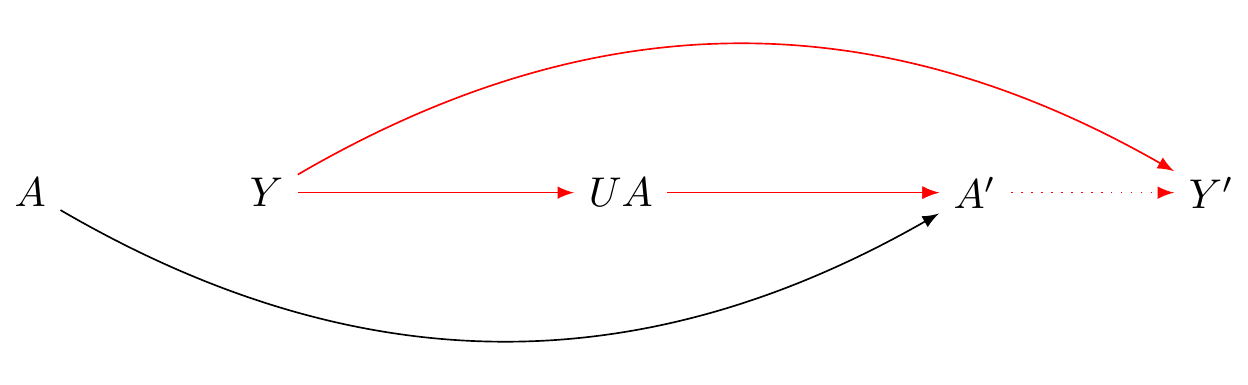
\includegraphics[width=1\textwidth,height=\textheight]{test-again_files/figure-pdf/fig-dag-measure-selection-0-1.pdf}

}

\caption{\label{fig-dag-measure-selection-0}The figure illustrates the
bias emanating from the outcome, Y, impacting the measurement error, UA,
of the documented exposure, A. While A and Y are independent, their
measured counterparts, A' and Y', are not. The systematic error
introduced in the historical recording opens a biasing path, signified
in red.}

\end{figure}

Figure~\ref{fig-dag-measure-selection} exposes the structure of bias
where post-outcome adjustment is necessary to mitigate or eliminate
measurement bias instigated by the outcome itself. Assume our interest
lies in quantifying the influence of belief in Big gods on social
complexity. We assumed that highly complex societies amend history,
eliminating traces of beliefs in lesser gods. If traces of beliefs in
lesser gods were recoverable through sources like language, we research
would obtain better effect estimates. The figure clarifies the intuition
that recovering ``echoes of the silenced'' is worthwhile for enhancing
the accuracy of our causal effect estimates.

\begin{figure}

{\centering 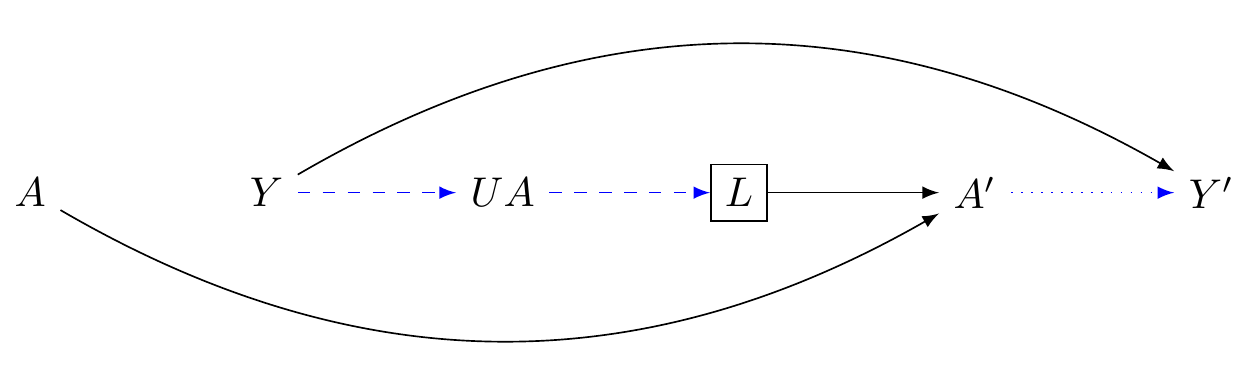
\includegraphics[width=1\textwidth,height=\textheight]{test-again_files/figure-pdf/fig-dag-measure-selection-1.pdf}

}

\caption{\label{fig-dag-measure-selection}Causal diagram elucidates how
refined measurements attenuate bias. Blue dotted arrows represent paths
that reduce the effect of measurement error bias by recovering measures
of the distorted exposure.}

\end{figure}

\hypertarget{refs}{}
\begin{CSLReferences}{1}{0}
\leavevmode\vadjust pre{\hypertarget{ref-mathur2018}{}}%
Mathur, Maya B, Peng Ding, Corinne A Riddell, and Tyler J VanderWeele.
2018. {``Website and r Package for Computing e-Values.''}
\emph{Epidemiology (Cambridge, Mass.)} 29 (5): e45.

\end{CSLReferences}



\end{document}
